\chapter{Iteration 3 (FYP-2 Mid)}
\label{ch:iter3}

The first iteration is expected to be completed by the midterm of the FYP-2.
This chapter will have some of the artifacts based on system design. The requirements analysis section is same for all the systems while the design may vary. There may have two types of designs the structural design or . First section is for the structural design.


\section{FYP-2 Mid}
\textbf{Objectives for FYP-2 Mid}
	\begin{itemize}
		\item Add basic tools related to Medical 
		\item User movements
		\item Patient Information
		\item Medicines Information 
	\end{itemize}
\newpage
\subsection{Tools and Medicines}
\text{We added some basic tools and medicines for practice.}
\begin{figure}[h]
	\centering
	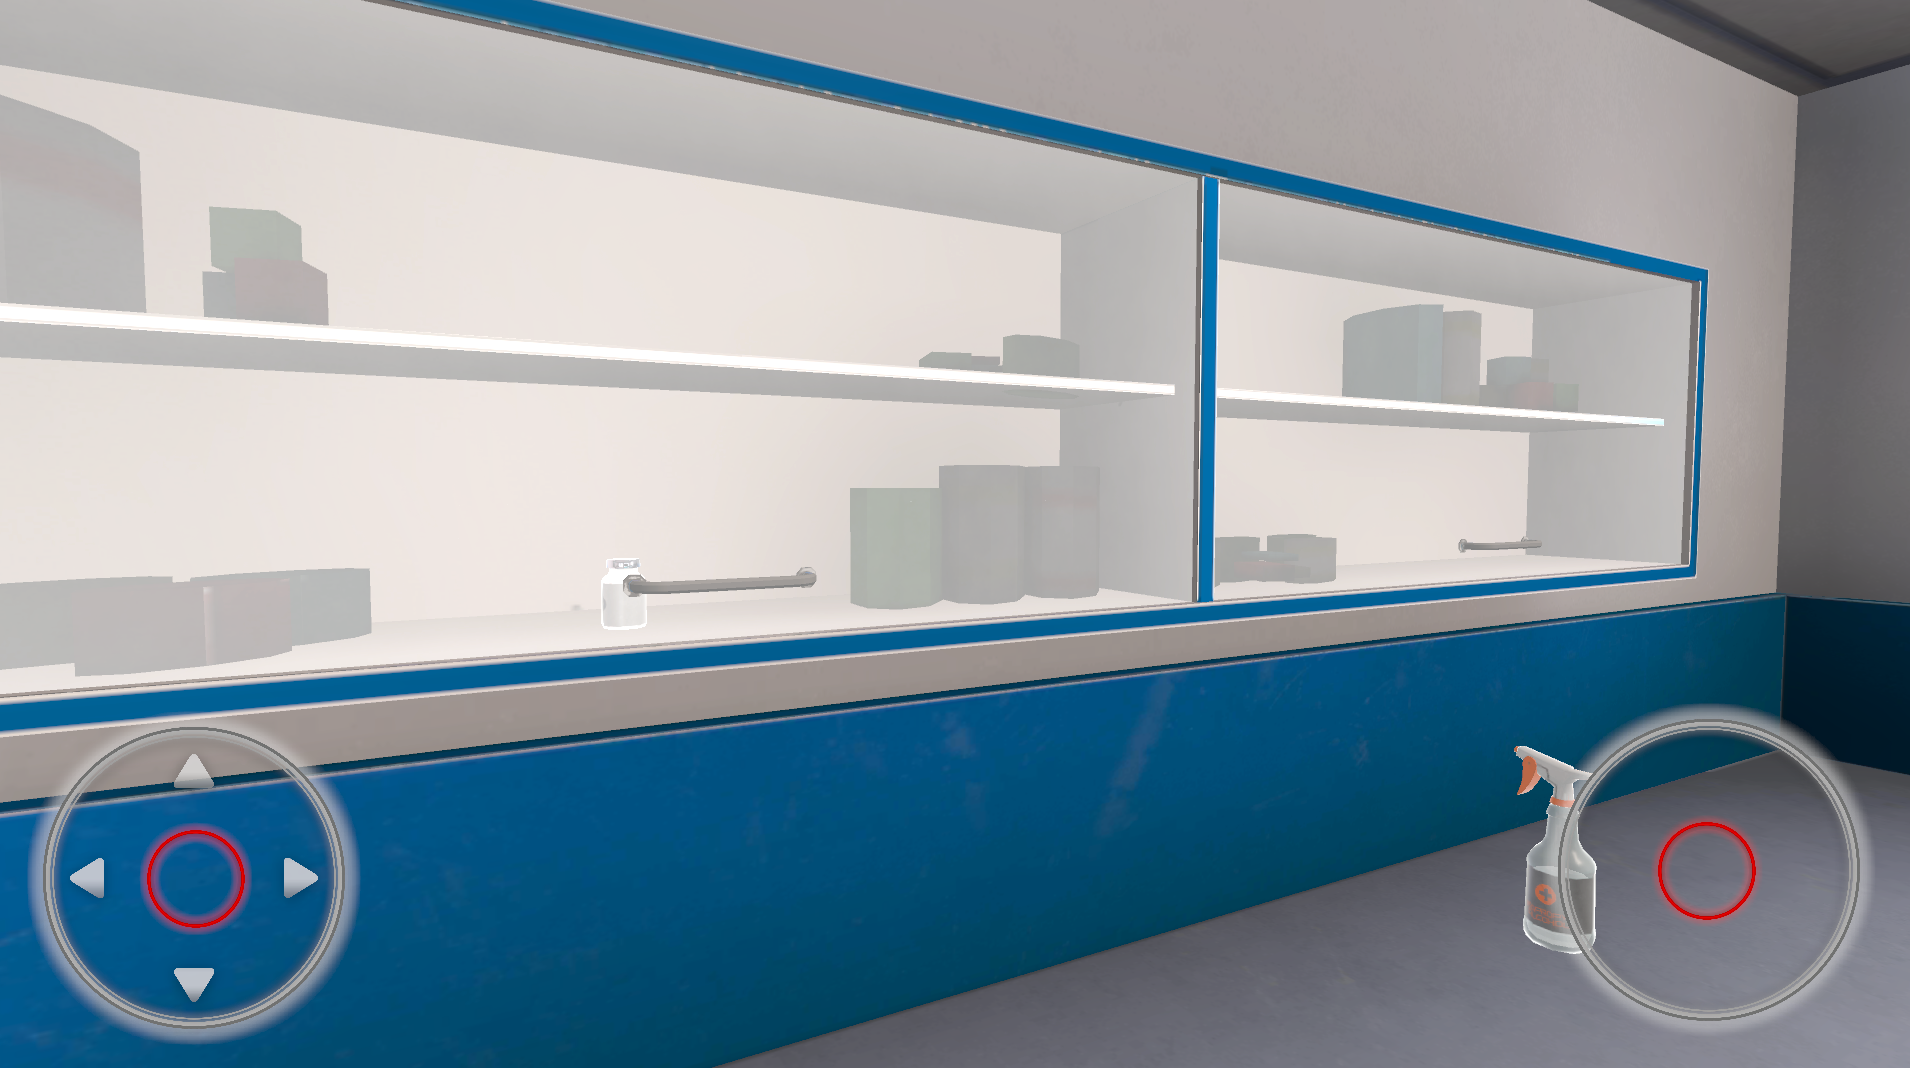
\includegraphics[width=0.65\linewidth]{Images/Toosls and Medicine.png}
	\caption{Toosls and Medicine}
	\label{fig:system-diagram}
\end{figure}

\begin{figure}[ht]
	\centering
	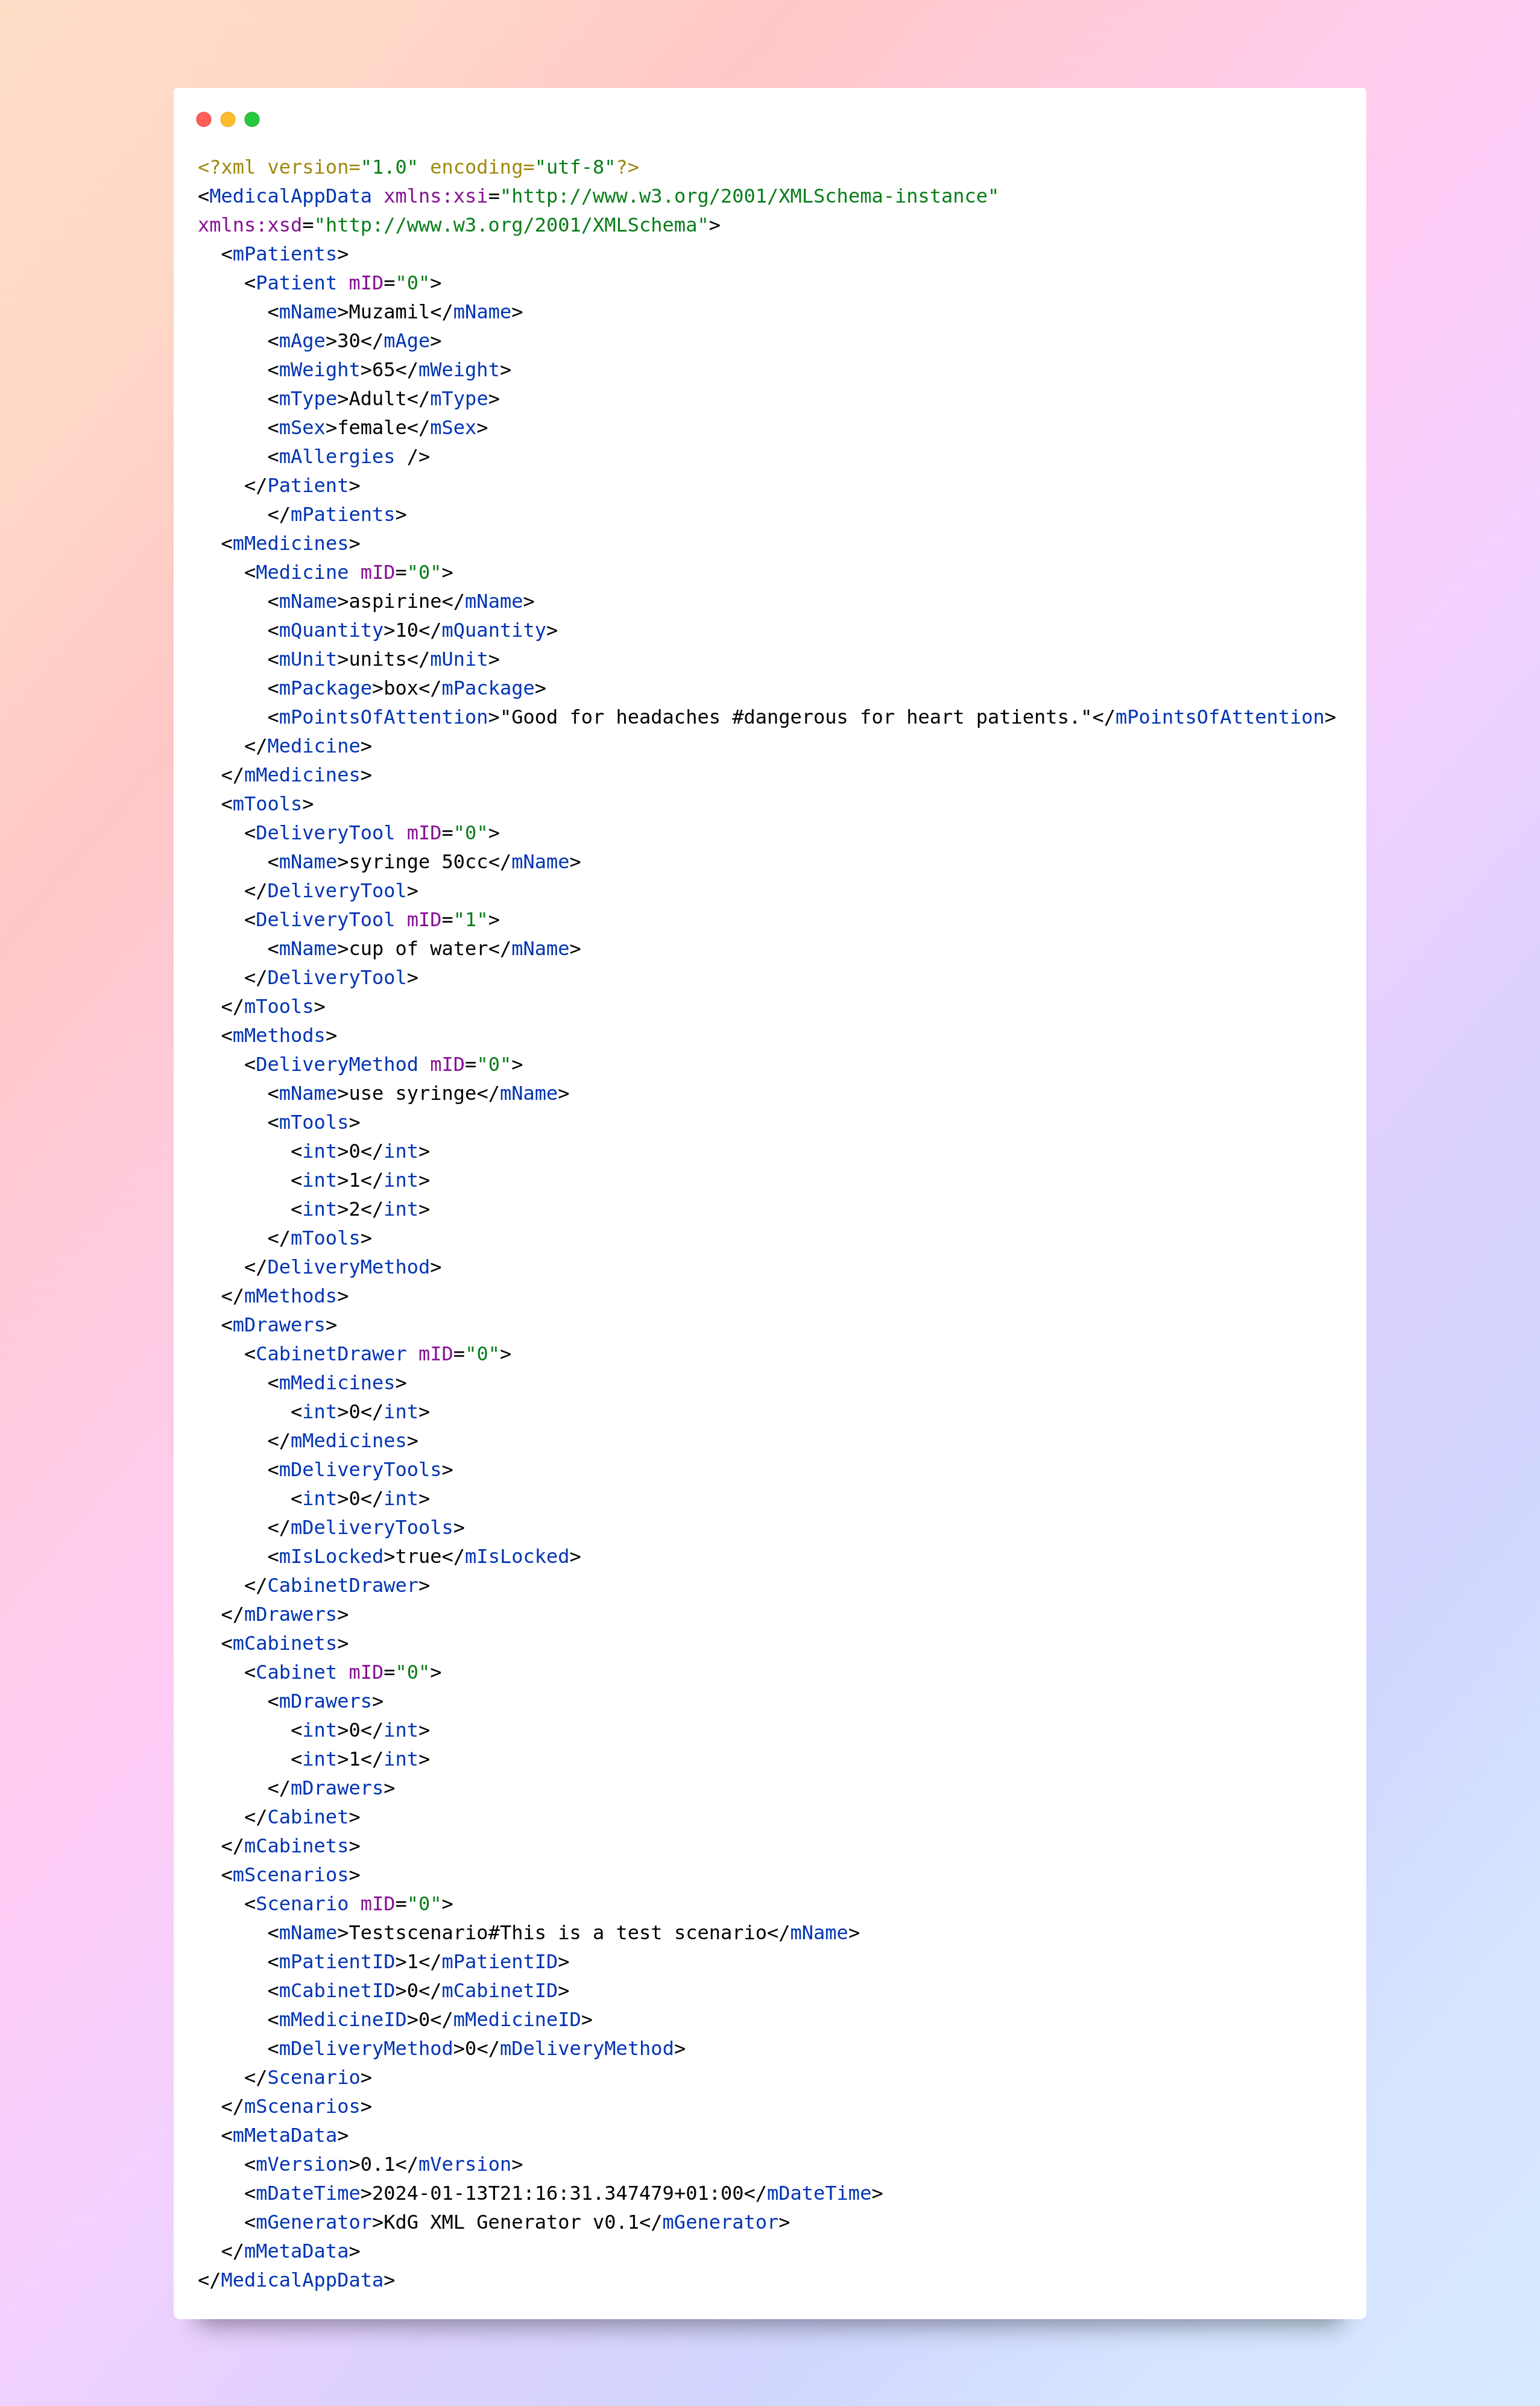
\includegraphics[width=1\linewidth, height=1.6\linewidth]{Images/medicines.png}
	\caption{Patient and Medicine Information code}
\end{figure}
\begin{figure}[ht]
	\centering
	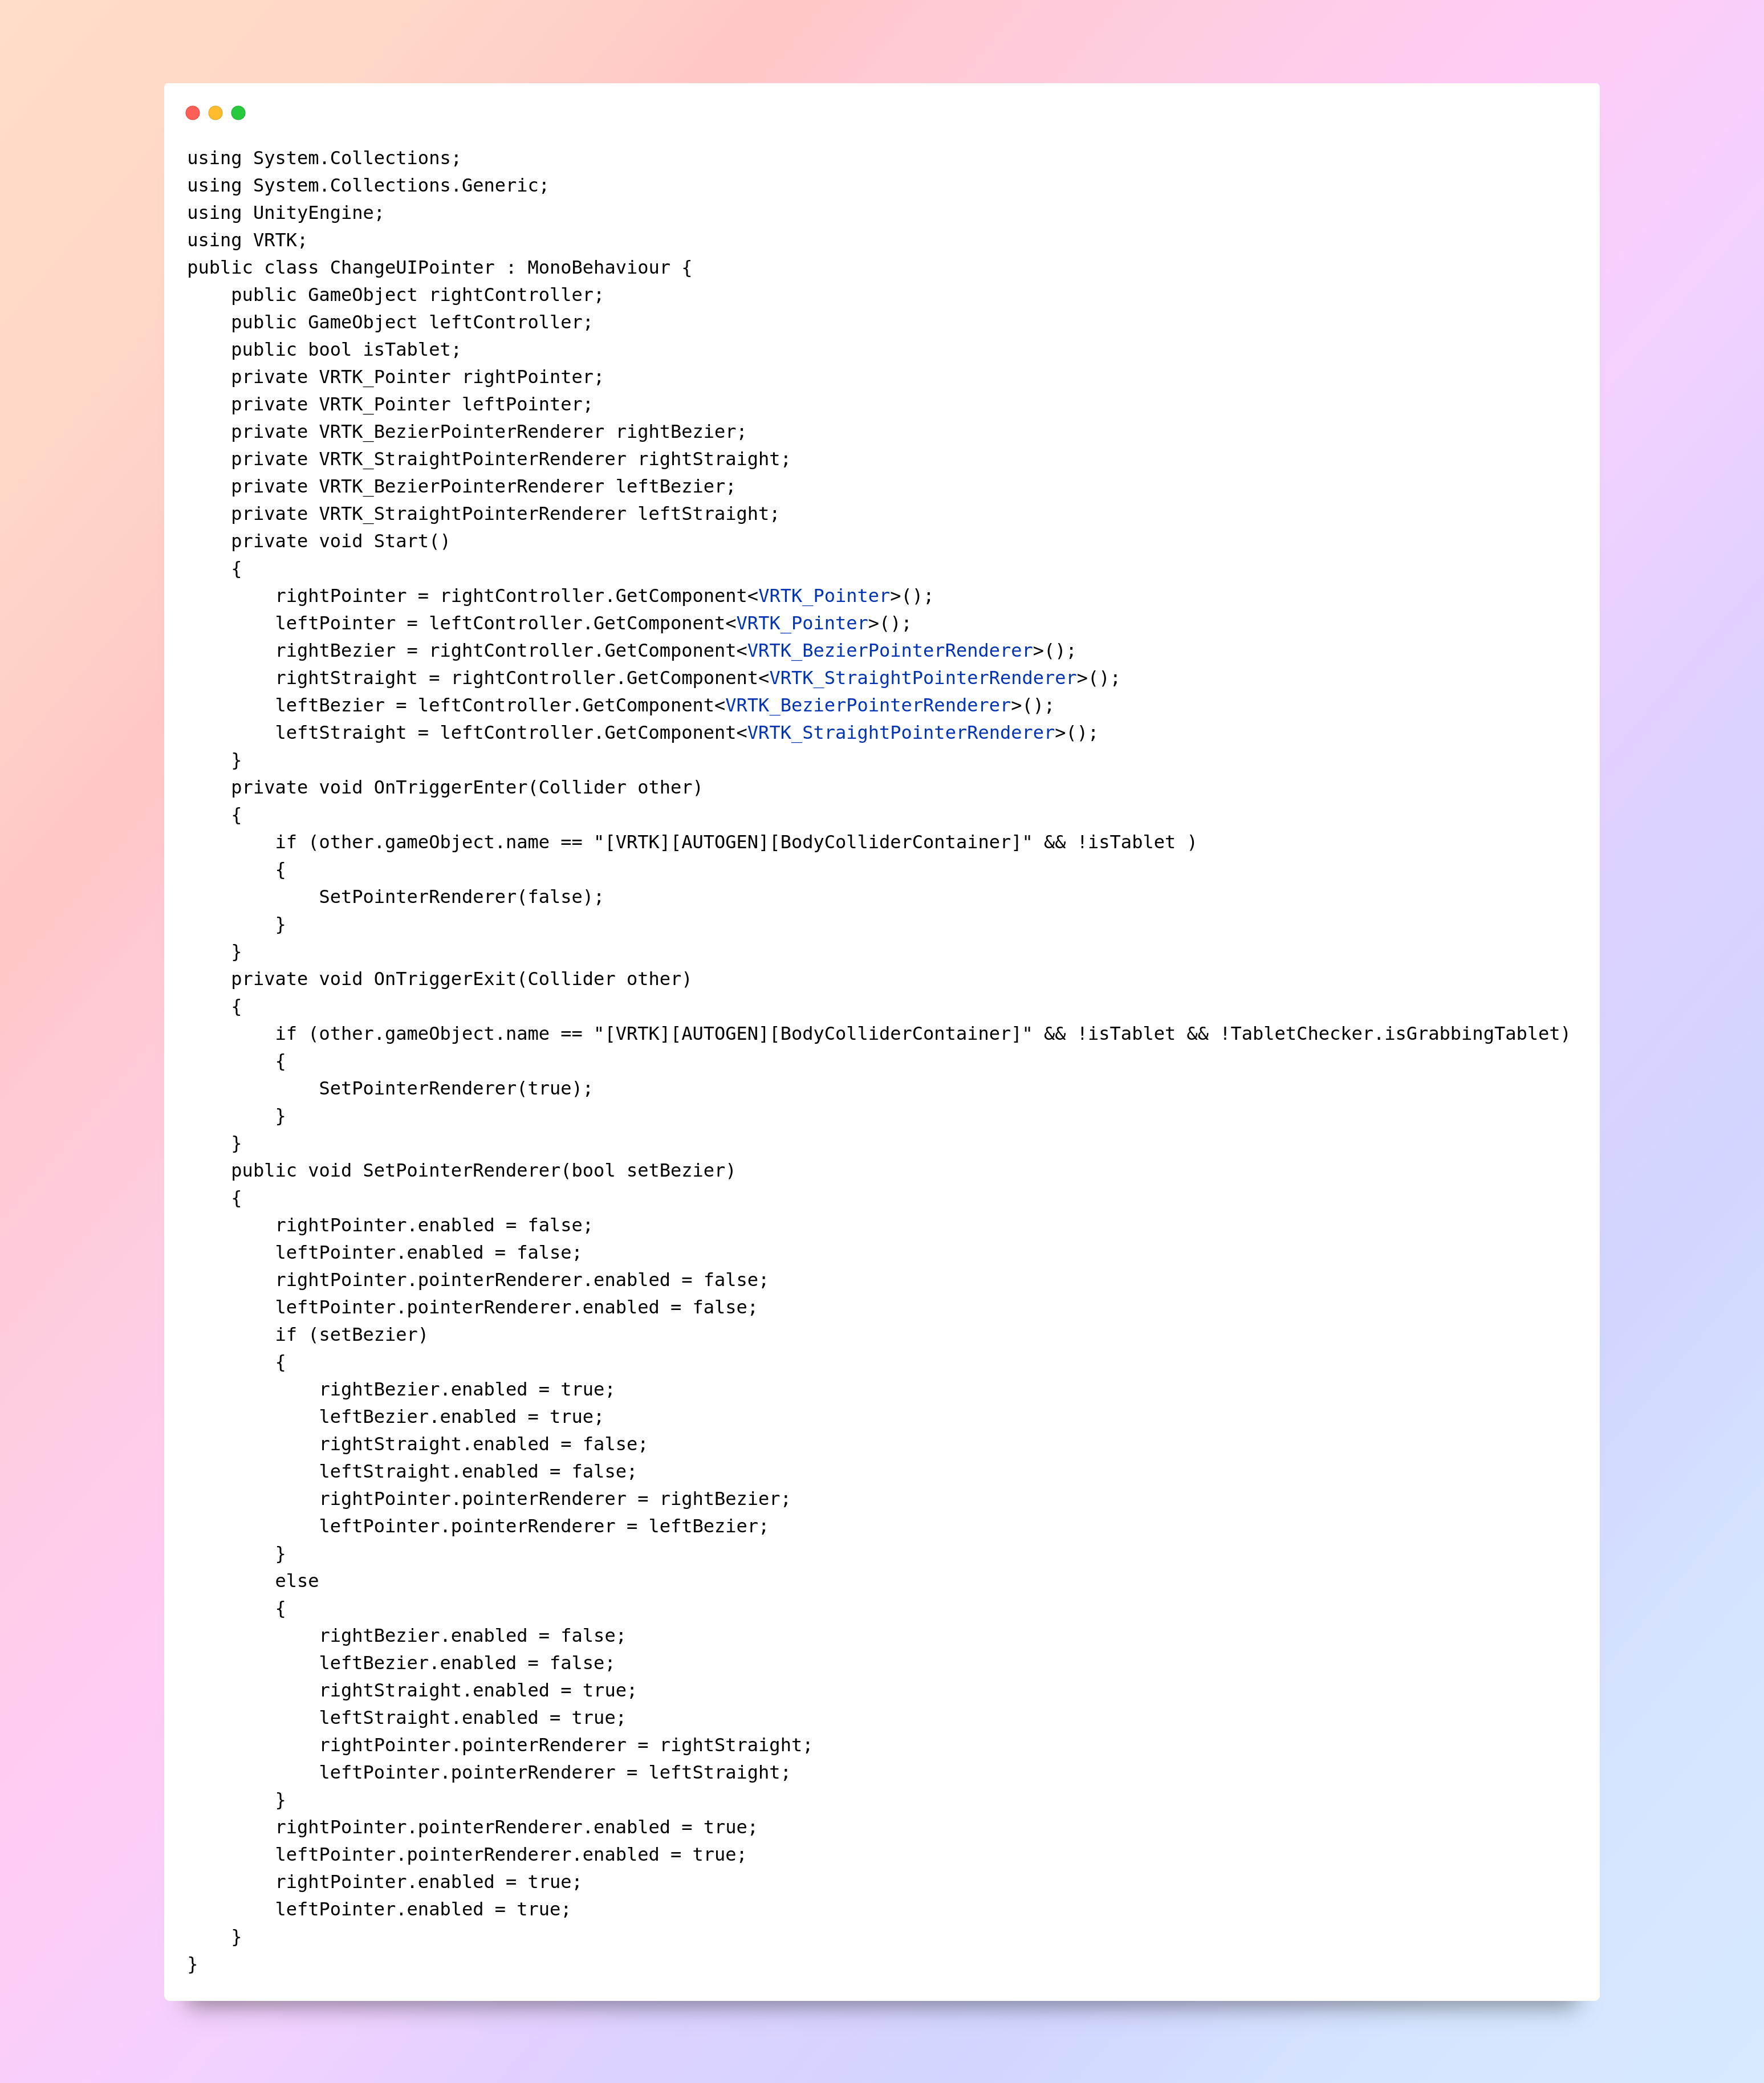
\includegraphics[width=1\linewidth, height=1.6\linewidth]{Images/ChangeUIPointer.png}
	\caption{Change UI Pointer code}
\end{figure}


\begin{figure}[ht]
	\centering
	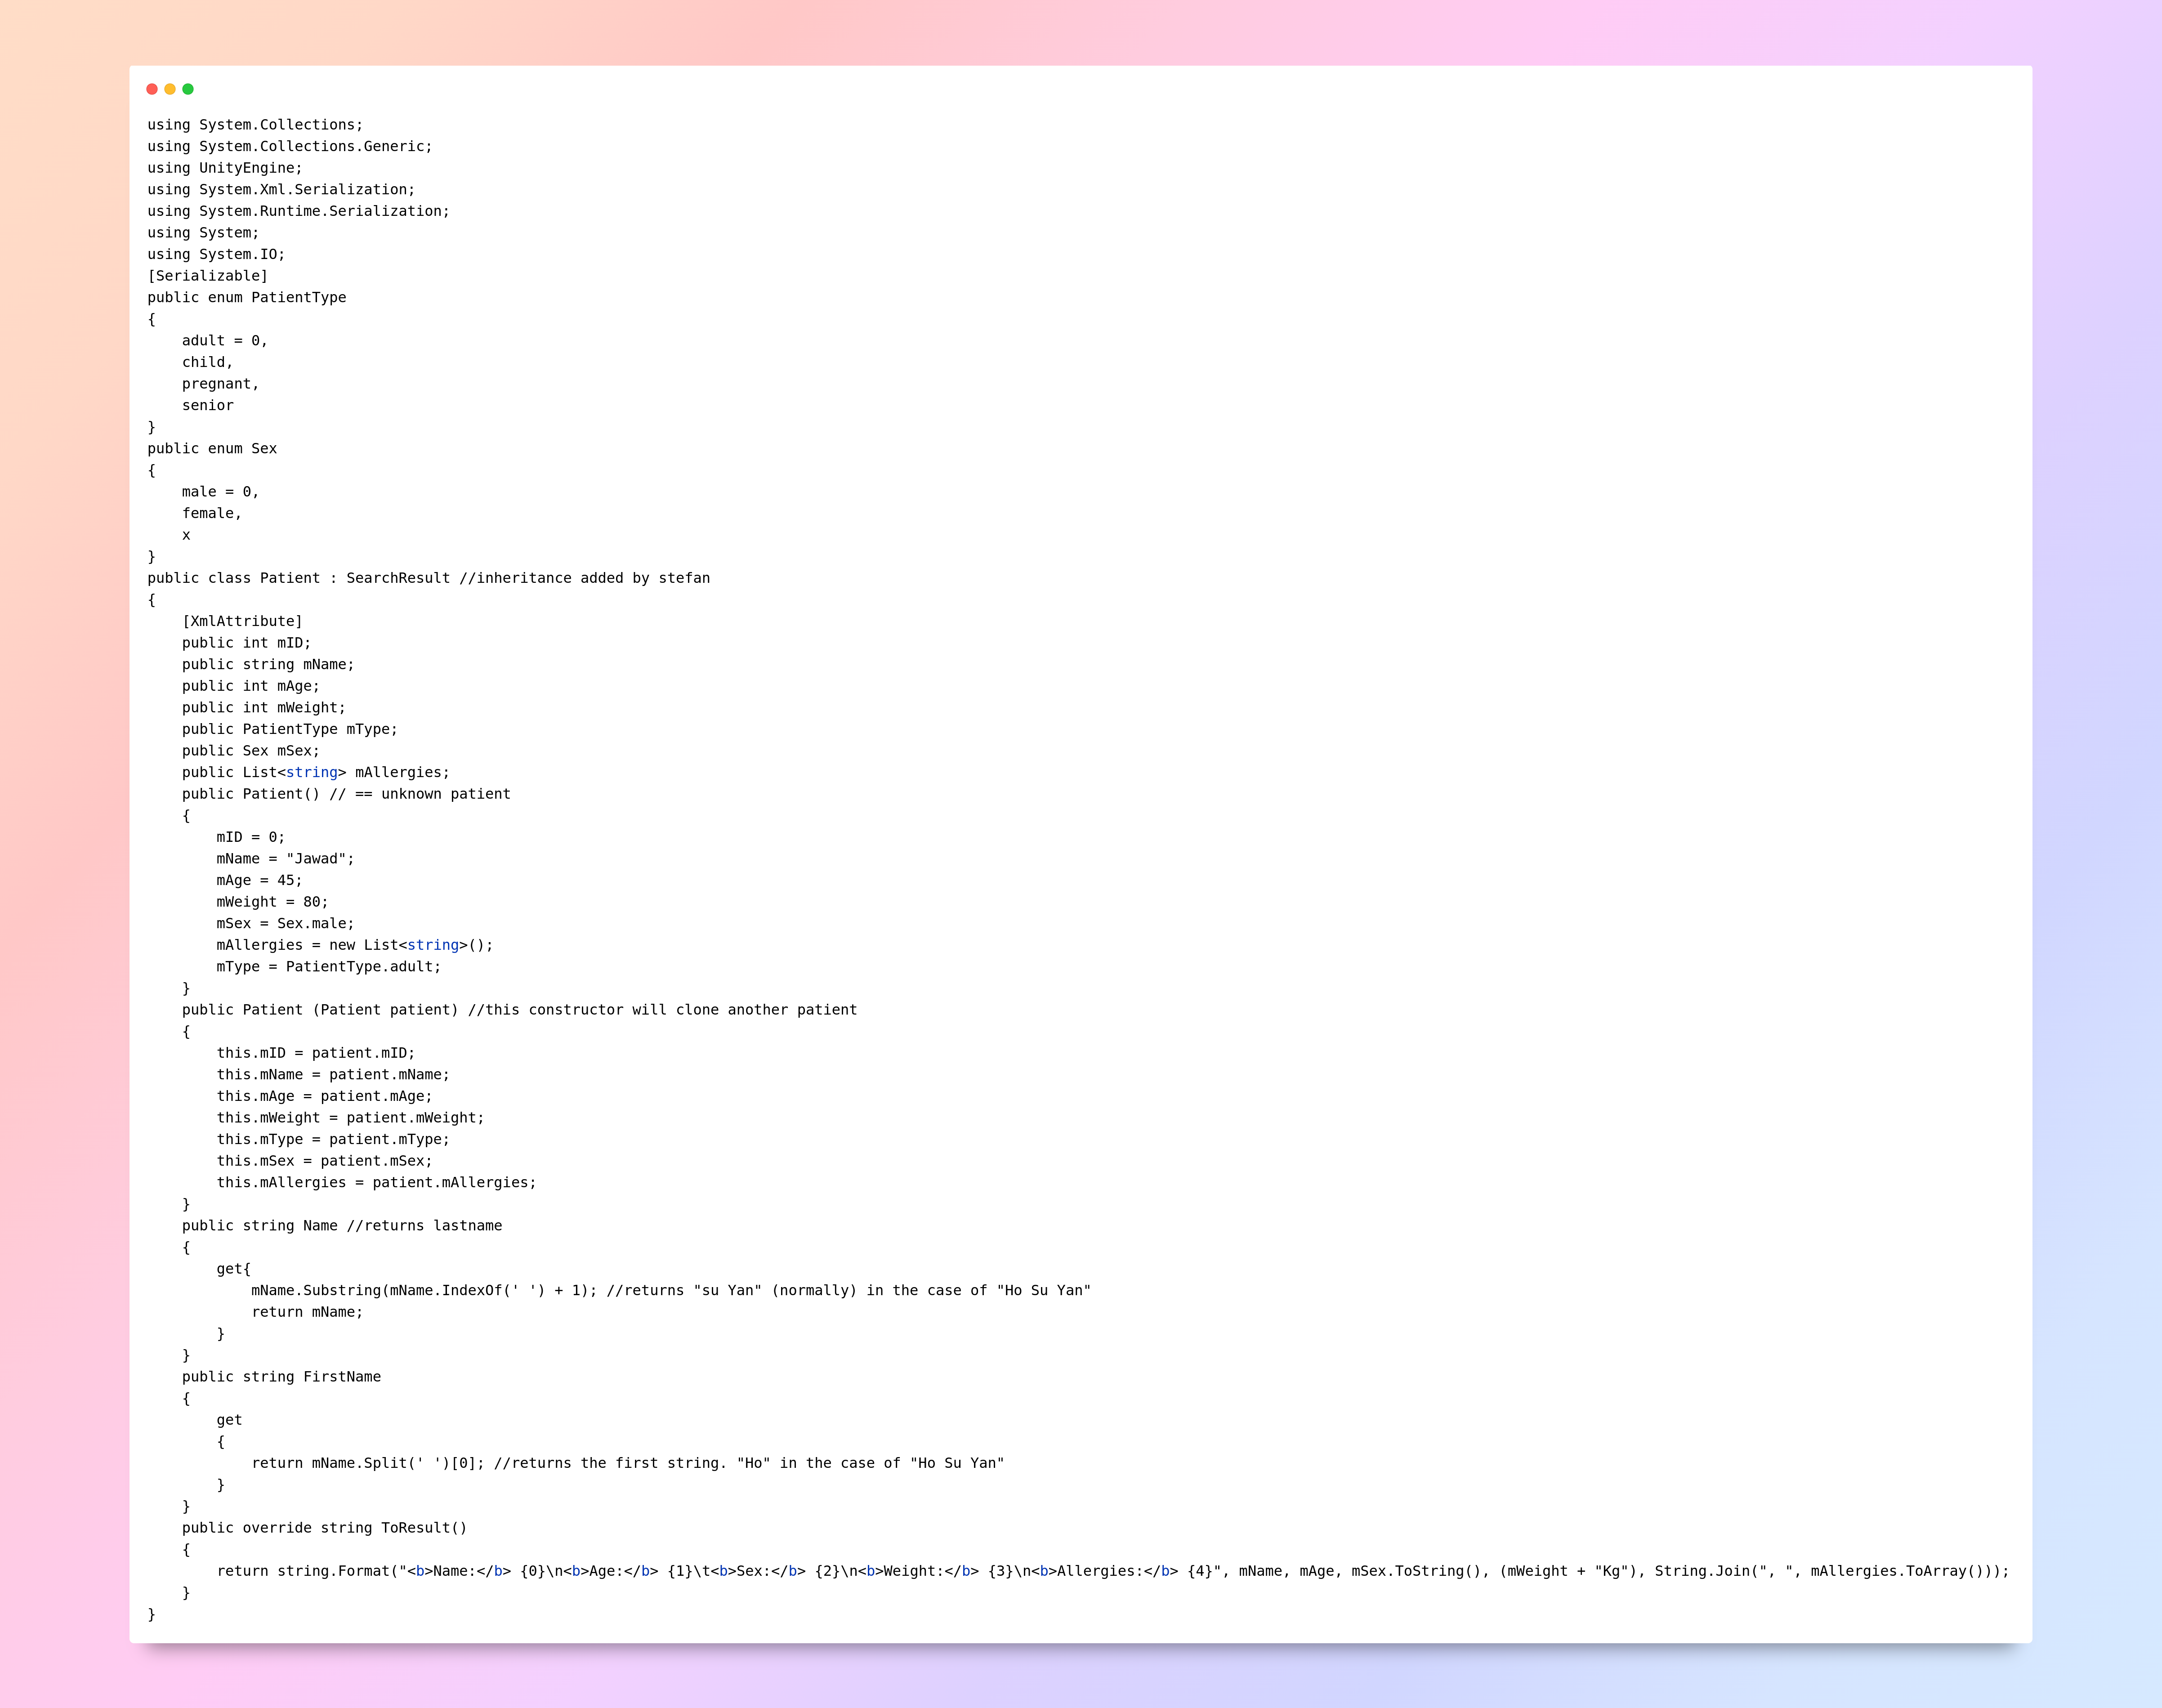
\includegraphics[width=1\linewidth, height=1\linewidth]{Images/patient.png}
	\caption{Patient Data code}
\end{figure}

\begin{figure}[ht]
	\centering
	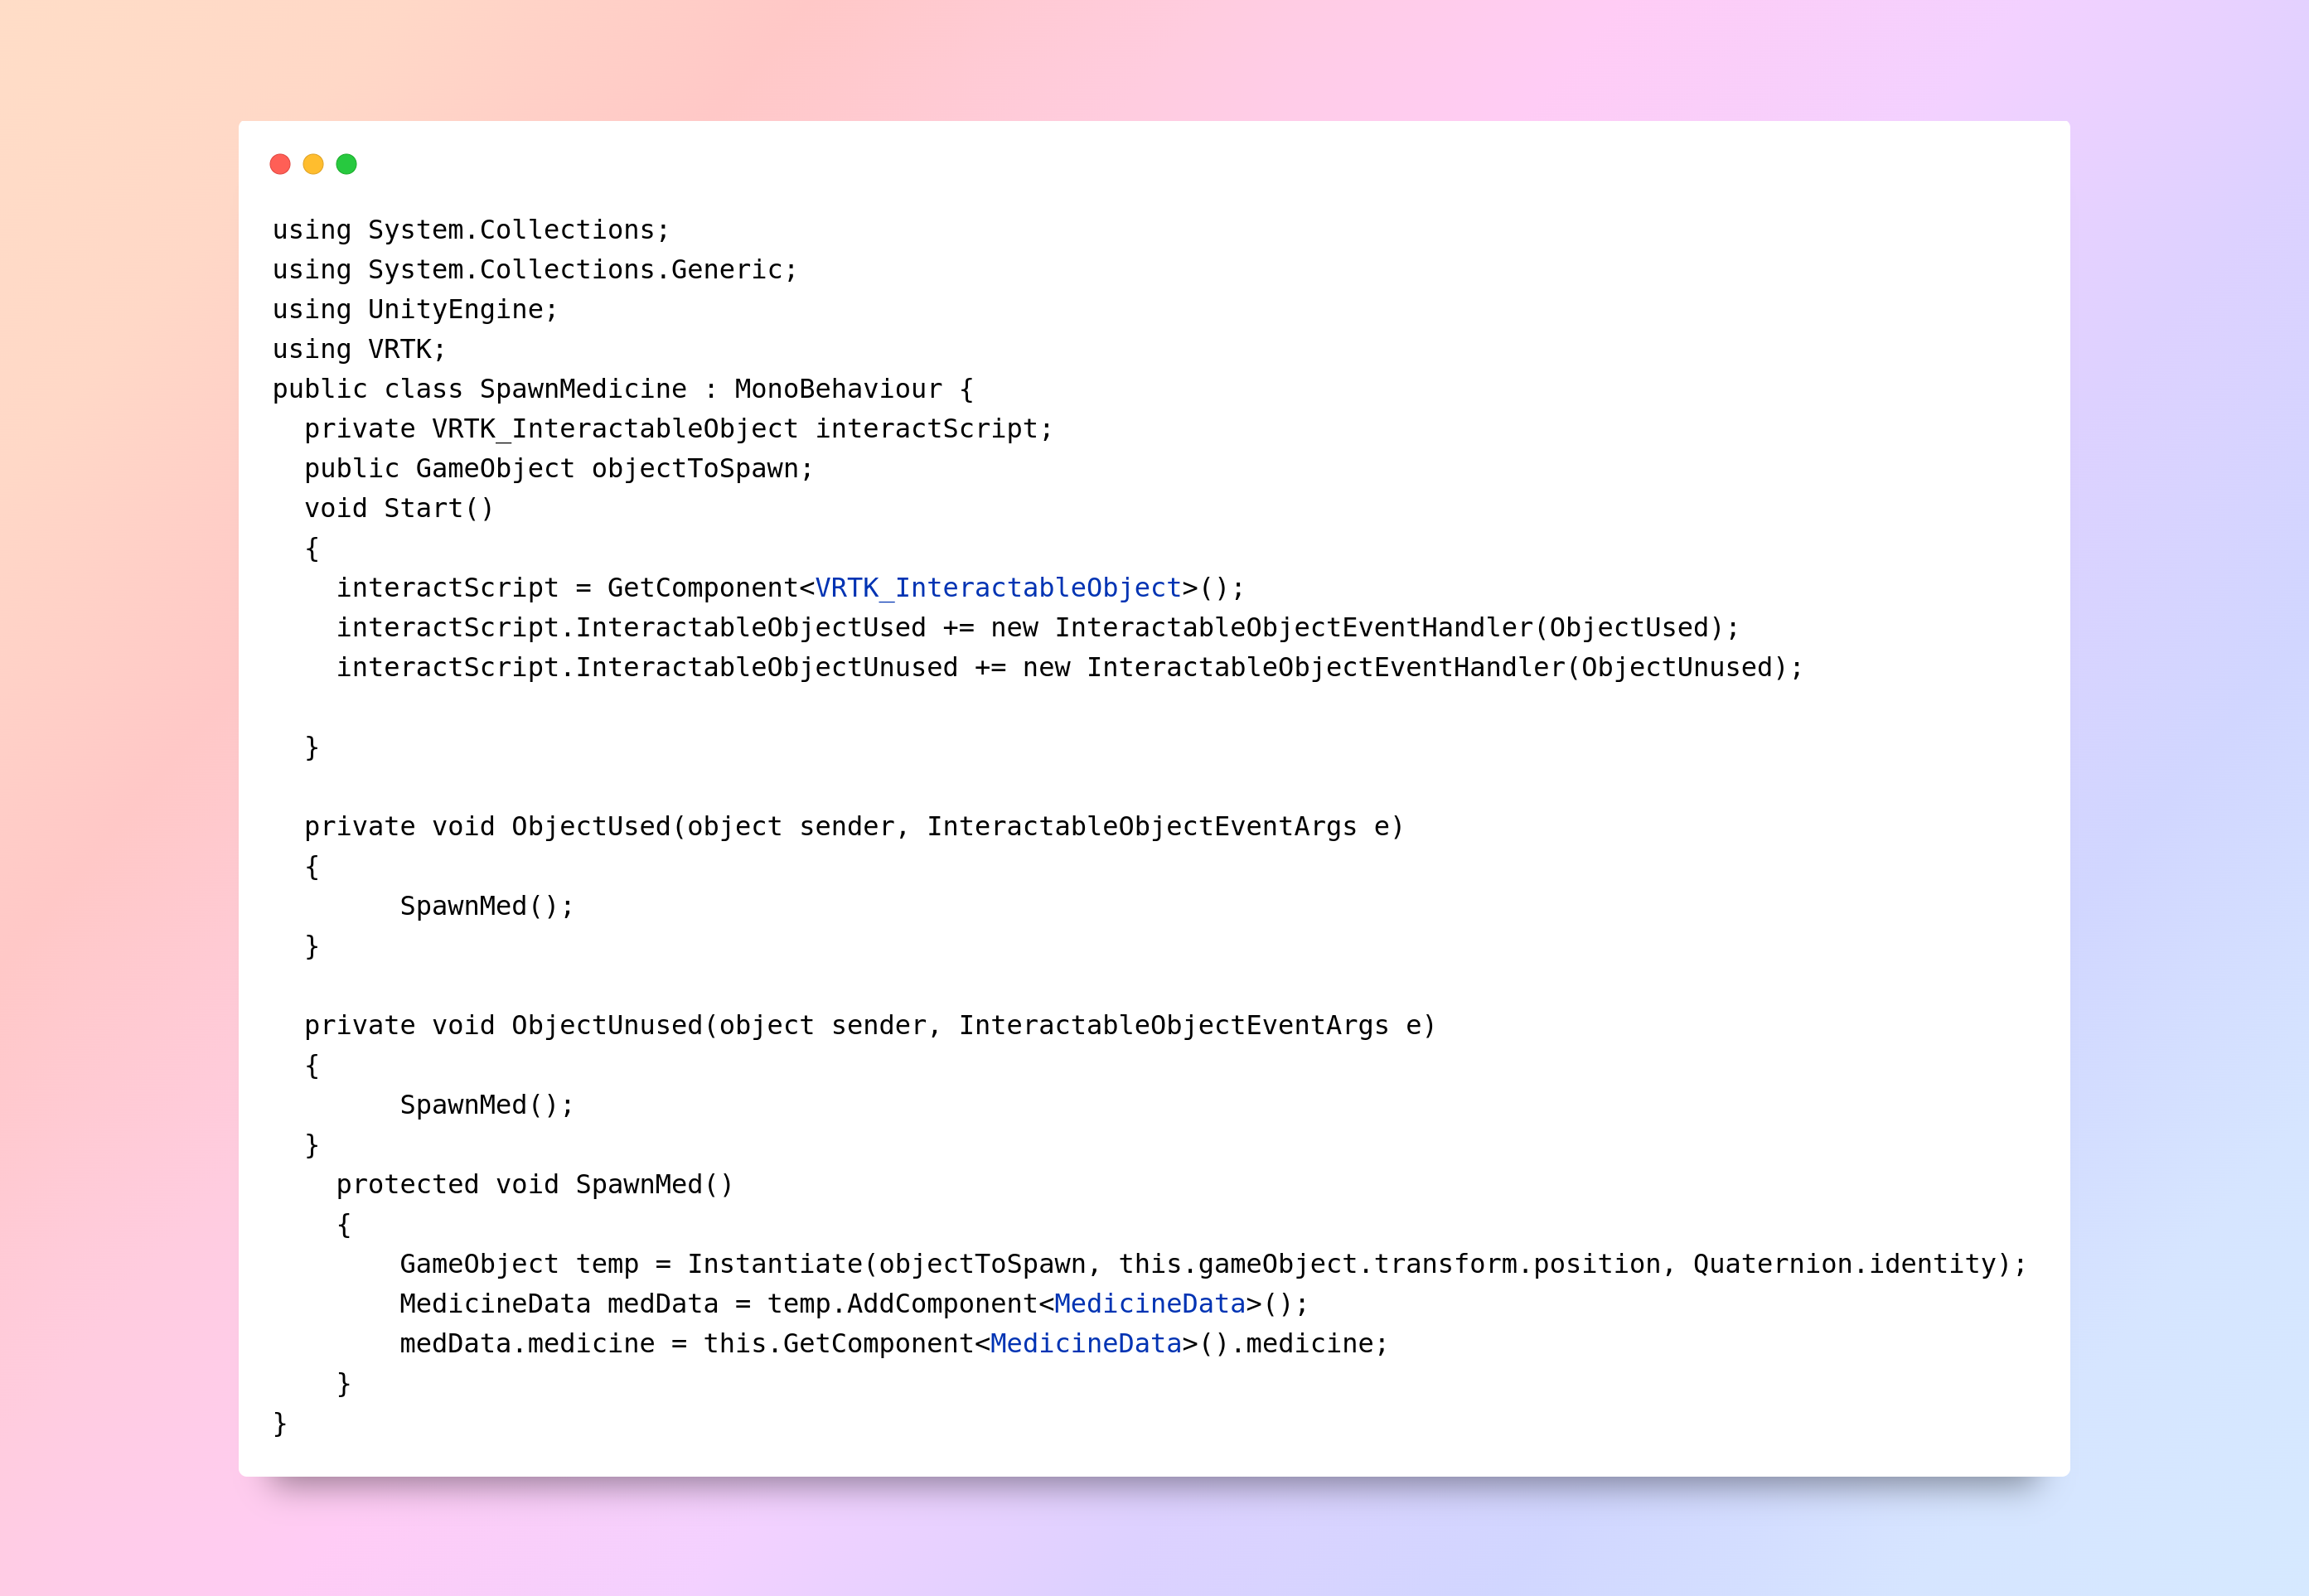
\includegraphics[width=1\linewidth, height=1\linewidth]{Images/SpwanMedicine.png}
	\caption{Spawn Medicine code}
\end{figure}


\begin{figure}[ht]
	\centering
	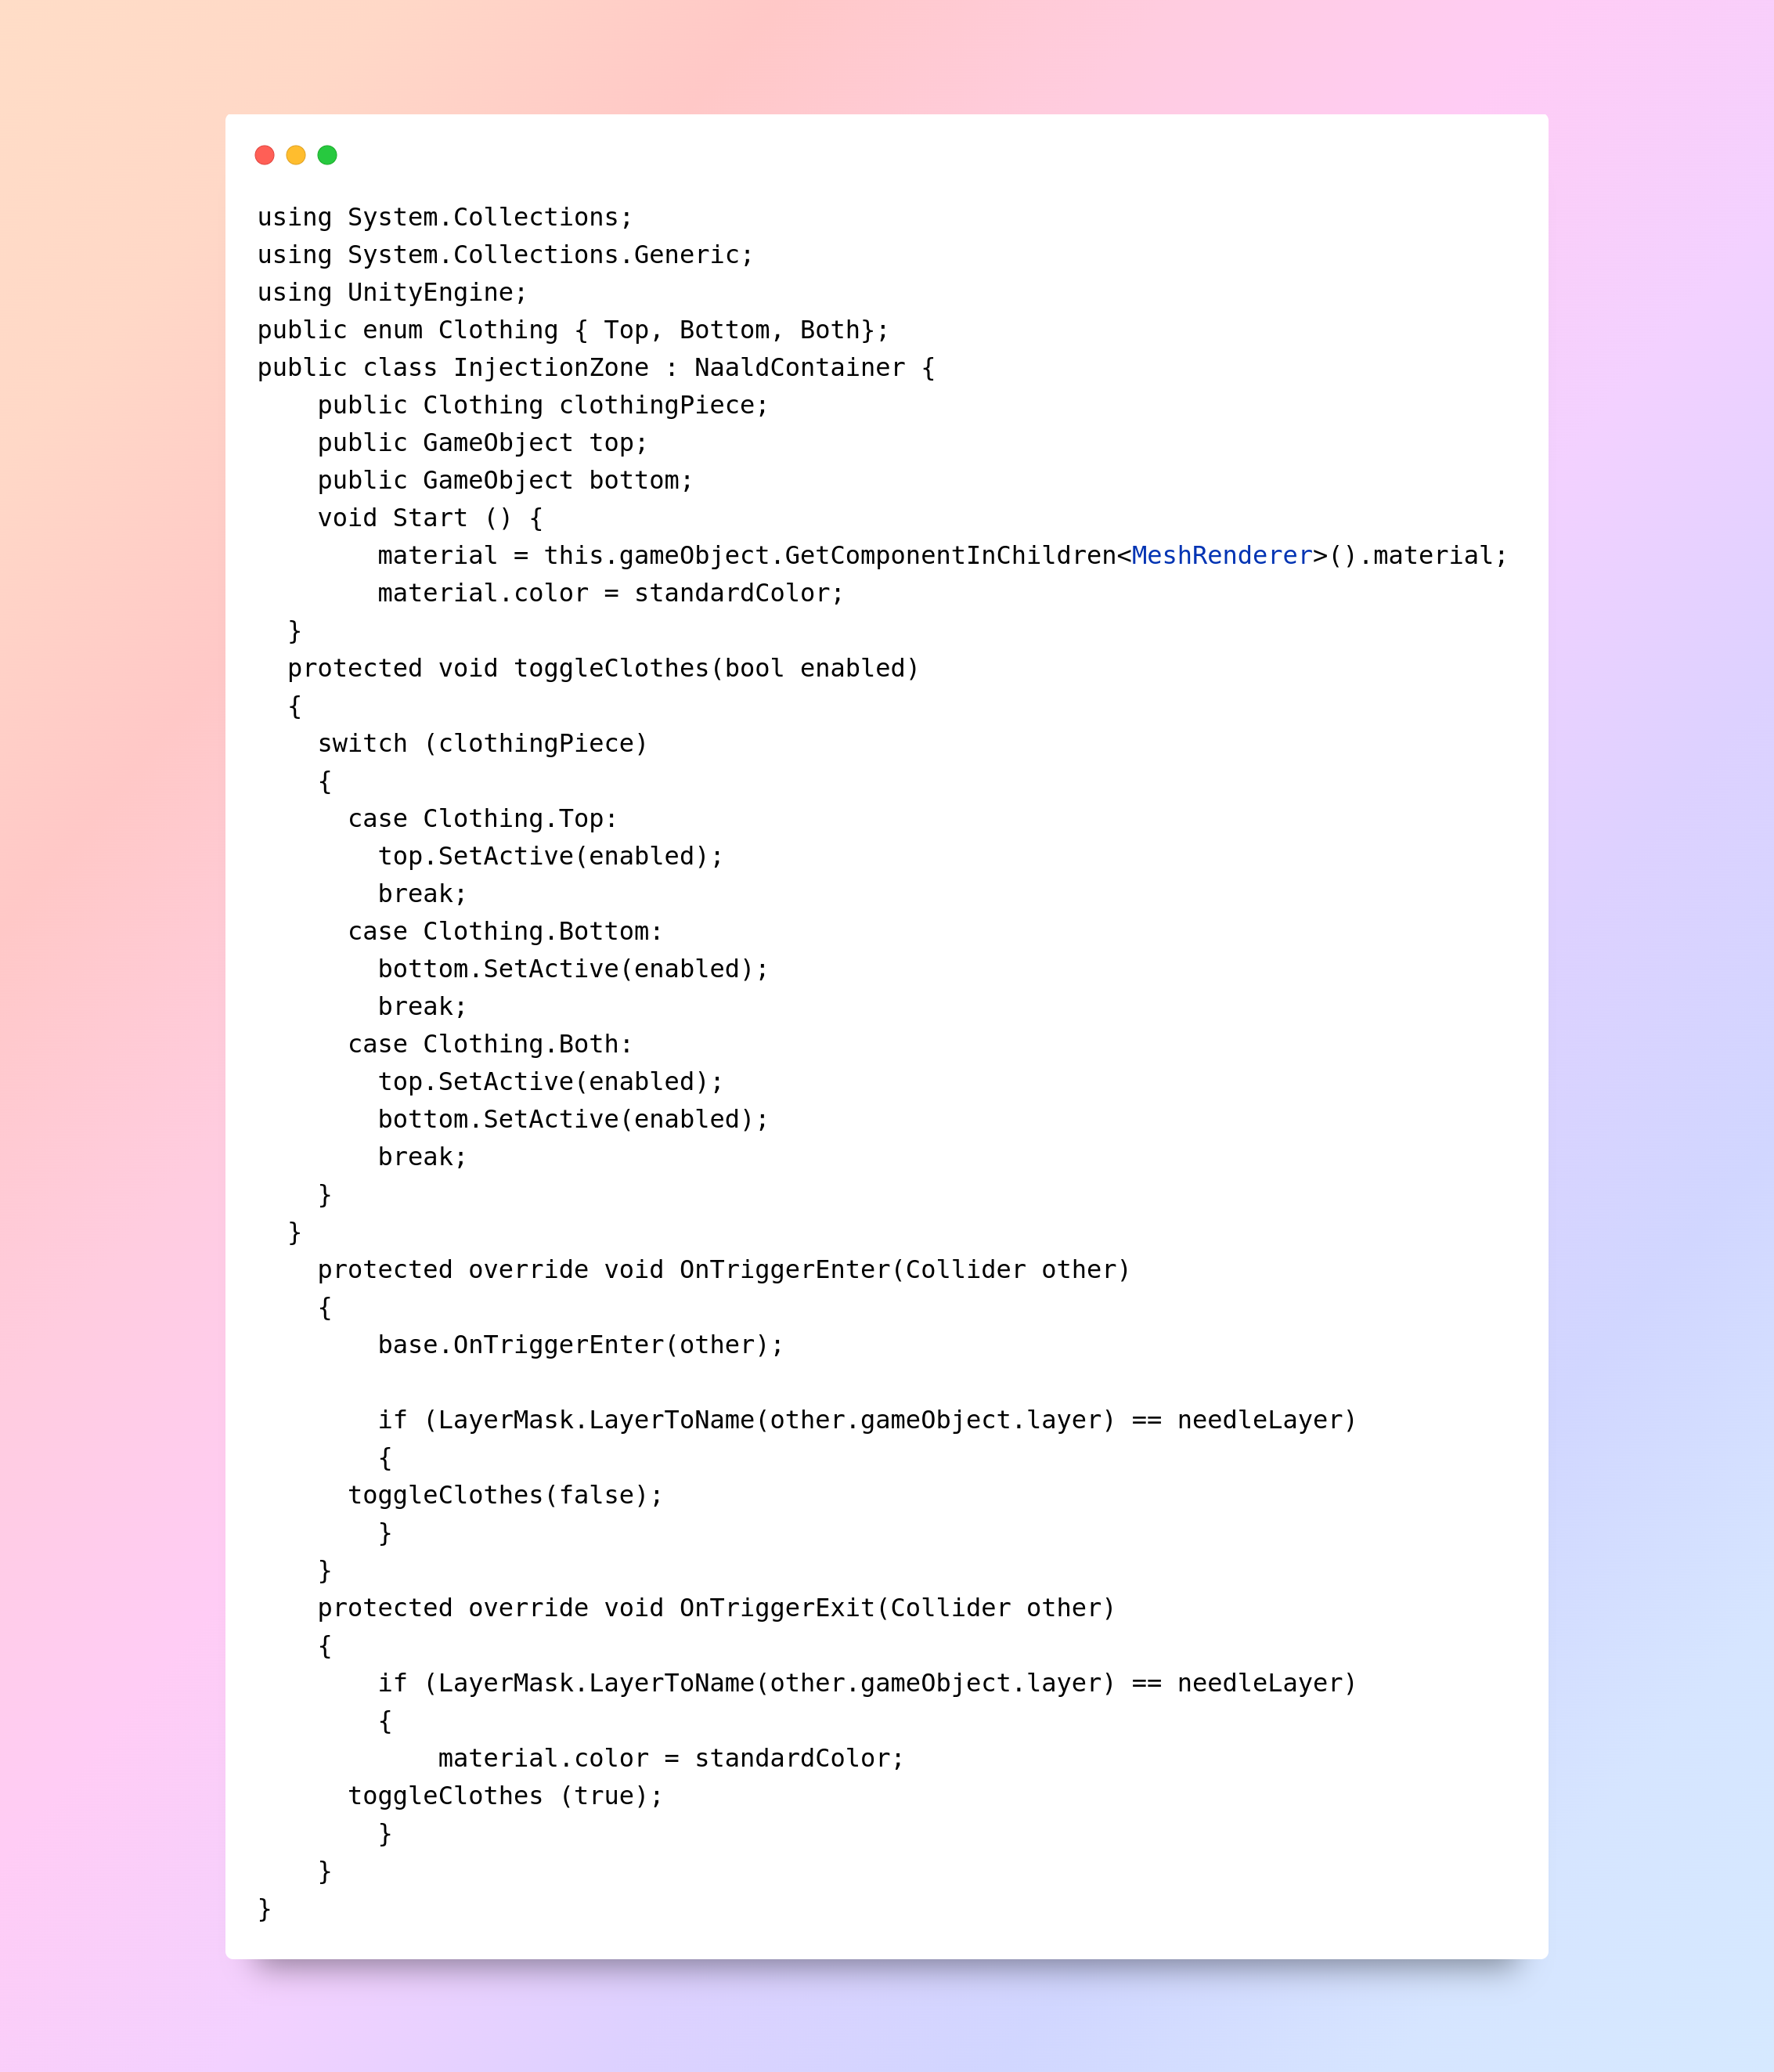
\includegraphics[width=1\linewidth, height=1.1\linewidth]{Images/Injection.png}
	\caption{Injection code}
\end{figure}

\section{SVN or GitHub}
We have uploaded on GitHub. Here is the GitHub link: \\
\href{https://github.com/Daudsarfraz/MetaMed}{https://github.com/Daudsarfraz/MetaMed}